\documentclass[a4paper, 12pt]{article}
% packages
\usepackage{amssymb}
\usepackage[fleqn]{mathtools}
\usepackage{tikz}
\usepackage{enumerate}
\usepackage{bussproofs}
\usepackage{xcolor}
\usepackage[margin=1.3cm]{geometry}
\usepackage{logicproof}
\usepackage{diagbox}
\usepackage{listings}
\usepackage{graphicx}
\usepackage{lstautogobble}
\usepackage{hyperref}
\usepackage{multirow}
\usetikzlibrary{arrows, shapes.gates.logic.US, circuits.logic.US, calc, automata, positioning}

% shorthand for verbatim
\catcode`~=\active
\def~#1~{\texttt{#1}}

% code listing
\lstdefinestyle{main}{
    numberstyle=\tiny,
    breaklines=true,
    showspaces=false,
    showstringspaces=false,
    tabsize=2,
    numbers=left,
    basicstyle=\ttfamily,
    columns=fixed,
    fontadjust=true,
    basewidth=0.5em,
    autogobble,
    xleftmargin=3.0ex,
    mathescape=true
}
\newcommand{\dollar}{\mbox{\textdollar}} %
\lstset{style=main}

% augmented matrix
\makeatletter
\renewcommand*\env@matrix[1][*\c@MaxMatrixCols c]{%
\hskip -\arraycolsep
\let\@ifnextchar\new@ifnextchar
\array{#1}}
\makeatother

% ceiling / floor
\DeclarePairedDelimiter{\ceil}{\lceil}{\rceil}
\DeclarePairedDelimiter{\floor}{\lfloor}{\rfloor}

% custom commands
\newcommand{\indefint}[2]{\int #1 \, \mathrm{d}#2}
\newcommand{\defint}[4]{\int_{#1}^{#2} #3 \, \mathrm{d}#4}
\newcommand{\dif}[2]{\frac{\mathrm{d}#1}{\mathrm{d}#2}}
\newcommand{\limit}[2]{\displaystyle{\lim_{#1 \to #2}}}
\newcommand{\summation}[3]{\sum\limits_{#1}^{#2} #3}
\newcommand{\intbracket}[3]{\left[#3\right]_{#1}^{#2}}
\newcommand{\ulsmash}[1]{\underline{\smash{#1}}}

\newcommand{\powerset}[0]{\wp}
\renewcommand{\emptyset}[0]{\varnothing}

\newcommand{\unaryproof}[2]{\AxiomC{#1} \UnaryInfC{#2} \DisplayProof}
\newcommand{\binaryproof}[3]{\AxiomC{#1} \AxiomC{#2} \BinaryInfC{#3} \DisplayProof}
\newcommand{\trinaryproof}[4]{\AxiomC{#1} \AxiomC{#2} \AxiomC{#3} \TrinaryInfC{#4} \DisplayProof}

% no indent
\setlength\parindent{0pt}

% reasoning proofs
\usepackage{ltablex}
\usepackage{environ}
\keepXColumns
\NewEnviron{reasoning}{
    \begin{tabularx}{\textwidth}{rlX}
        \BODY
    \end{tabularx}
}
\newcommand{\proofline}[3]{$(#1)$ & $#2$ & \hfill #3 \smallskip \\}
\newcommand{\proofarbitrary}[1]{& take arbitrary $#1$ \smallskip \\}
\newcommand{\prooftext}[1]{\multicolumn{3}{l}{#1} \smallskip \\}
\newcommand{\proofmath}[3]{$#1$ & = $#2$ & \hfill #3 \smallskip \\}
\newcommand{\prooftherefore}[1]{& $\therefore #1$ \smallskip \\}
\newcommand{\proofbc}[0]{\prooftext{\textbf{Base Case}}}
\newcommand{\proofis}[0]{\prooftext{\textbf{Inductive Step}}}

% reasoning er diagrams
\newcommand{\nattribute}[4]{
    \node[draw, state, inner sep=0cm, minimum size=0.2cm, label=#3:{#4}] (#1) at (#2) {};
}
\newcommand{\mattribute}[4]{
    \node[draw, state, accepting, inner sep=0cm, minimum size=0.2cm, label=#3:{#4}] (#1) at (#2) {};
}
\newcommand{\dattribute}[4]{
    \node[draw, state, dashed, inner sep=0cm, minimum size=0.2cm, label=#3:{#4}] (#1) at (#2) {};
}
\newcommand{\entity}[3]{
    \node[] (#1-c) at (#2) {#3};
    \node[inner sep=0cm] (#1-l) at ($(#1-c) + (-1, 0)$) {};
    \node[inner sep=0cm] (#1-r) at ($(#1-c) + (1, 0)$) {};
    \node[inner sep=0cm] (#1-u) at ($(#1-c) + (0, 0.5)$) {};
    \node[inner sep=0cm] (#1-d) at ($(#1-c) + (0, -0.5)$) {};
    \draw
    ($(#1-c) + (-1, 0.5)$) -- ($(#1-c) + (1, 0.5)$) -- ($(#1-c) + (1, -0.5)$) -- ($(#1-c) + (-1, -0.5)$) -- cycle;
}
\newcommand{\relationship}[3]{
    \node[] (#1-c) at (#2) {#3};
    \node[inner sep=0cm] (#1-l) at ($(#1-c) + (-1, 0)$) {};
    \node[inner sep=0cm] (#1-r) at ($(#1-c) + (1, 0)$) {};
    \node[inner sep=0cm] (#1-u) at ($(#1-c) + (0, 1)$) {};
    \node[inner sep=0cm] (#1-d) at ($(#1-c) + (0, -1)$) {};
    \draw
    ($(#1-c) + (-1, 0)$) -- ($(#1-c) + (0, 1)$) -- ($(#1-c) + (1, 0)$) -- ($(#1-c) + (0, -1)$) -- cycle;
}

% actual document
\begin{document}
    \section*{CO130 - Databases}
        \subsection*{Prelude}
            The content discussed here is part of CO130 - Databases (Computing MEng); taught by Thomas Heinis, in Imperial College London during the academic year 2018/19. The notes are written for my personal use, and have no guarantee of being correct (although I hope it is, for my own sake).
        \subsection*{Material Order}
            These notes are primarily based off the slides on CATe. This is the order in which they are uploaded (and I'd assume the order in which they are taught).
            \begin{enumerate}[1.]
                \itemsep0em
                \item \textit{Introduction.pdf}
                \item \textit{ER Modelling.pdf}
                \item \textit{ER to RM.pdf}
                \item \textit{Relational Algebra.pdf}
                \item \textit{Tutorial ER.pdf}
                \item \textit{Tutorial Translation.pdf}
                \item \textit{Relational Algebra.pdf}
                \item \textit{Functional Dependencies.pdf}
                \item \textit{Tutorial Relational Algebra.pdf}
                \item \textit{Normalisation.pdf}
                \item \textit{SQL.pdf}
                \item \textit{Data Definition.pdf}
                \item \textit{Data Manipulation.pdf}
                \item \textit{Advanced SQL.pdf}
                \item \textit{Functional Dependency Tutorial.pdf}
                \item \textit{Transactions.pdf}
                \item \textit{SQL Tutorial.pdf}
                \item \textit{Storage.pdf}
                \item \textit{Indexing.pdf}
                \item \textit{NoSQL.pdf}
                \item \textit{MapReduce.pdf}
            \end{enumerate}
        \subsection*{Introduction}
            We use databases as it's more organised; hence it's easier to model and manage. It's more efficient, as it's fast to search, and update, and integration allows us to minimise data duplication. Concurrent (and therefore multi-user) access allows multiple people to access the database at the same time (will require some techniques).
            \medskip

            \textbf{Transactions} are sequences of database actions that execute in a coherent, and reliable way - the classical properties are \textbf{ACID}. Consider the two transactions ~T1~: $A = A - 100; B = B + 100$, and ~T2~: $B = B - 100; A = A + 100$, we can observe ACID properties as follows;
            \begin{itemize}
                \itemsep0em
                \item \textbf{atomicity} \hfill if one part of a transaction fails, the entire transaction fails
                    \subitem on completion of ~T1~, either $A^\prime = A - 100$, and $B^\prime = B + 100$, or $A^\prime = A$, and $B^\prime = B$, where the former is a successful transaction, and the latter is in the case of a failure.
                \item \textbf{consistency} \hfill transactions don't leave the database in an inconsistent state
                    \subitem the sum of the balances must remain the same, such that $A^\prime + B^\prime = A + B$; we can also have more constraints such as keeping balances positive, or limiting the amount a transfer can do at once
                \item \textbf{isolation} \hfill transactions run as if no other transactions are running (may need to wait)
                    \subitem given the two concurrent transactions ~T1~, and ~T2~, one has to be completed before the other can start
                \item \textbf{durability} \hfill results of successful transactions aren't lost on system failure
                    \subitem the new values, $A^\prime$, and $B^\prime$ must persist if the transaction completes, even if the system fails (disk failure etc.)
            \end{itemize}
            A \textbf{Database Management System (DMBS)} creates new databases via a \textbf{Data Definition Language (DDL)}, which specifies the structure (\textbf{schema}). It also queries, and manipulates through a \textbf{Data Manipulation Language (DML)}. Examples of this include \textit{PostgreSQL}, \textit{MySQL}, \textit{SQLite}, and can also fall under \textit{NoSQL}, however SQL remains as the most widespread technology (as of writing this).
            \medskip

            It lets us define, query, and manipulate databases with a high-level declarative language (\textbf{Structured Query Language}). It's standardised by the ISO, but each DBMS implements its own variation of the standards, which may be costly if it's complex.
            \subsubsection*{Relational Model}
                Consider the following model, represented as a table;
                \begin{center}
                    \begin{tabular}{|c|c|c|c|c|}
                        \hline
                        heading & ~title:string~ & ~year:int~ & ~length:int~ & ~genre:string~ \\
                        \hline
                        \hline
                        \multirow{3}{*}{body} & Gone with the Wind & 1939 & 231 & Drama \\
                        \cline{2-5}
                        & Star Wars & 1977 & 124 & Science Fiction \\
                        \cline{2-5}
                        & Luis' World & 1992 & 95 & Comedy \\
                        \hline
                    \end{tabular}
                \end{center}
                We have the columns be the attribute, with the top row being the heading, and the rest being the body. The attributes are in the format ~name:type~. The rows (of the body) are referred to as tuples. A relation is the heading as well as the body (the entire table). The heading is an \textbf{unordered set} of attributes, and an attribute is the name as well as the type (typically indivisible types). The body is an unordered set of tuples, and a tuple is the set of attribute values. The schema is for the entire relation is the name of the relation, and the heading, in this case, we'd have; ~movies(title:string, year:int, length:int, genre:string)~, and a database is a collection of relations. A schema for a database is the schemas for all relations.
                \medskip

                In mathematics, with a set of sets; $S_1, S_2, ..., S_n$, a relation $R$ is a set of tuples $T_1, T_2, ..., T_n$, where $T_k \in S_k$, therefore $R \subset S_1 \times S_2 \times ... \times S_n$. As the idea of relations stems from set theory, it's important to note that the order in which we represent the attributes, and tuples in unimportant. In the Relational model we have \textbf{attributed} tuples, rather than \textbf{ordered}; $R$ is the set of tuples ($A_1:S_1=T_1, ..., A_n:S_n=T_n$), with $T_k \in S_k$. It's important to note that relations aren't 2-dimensional tables, even though it's more convenient to draw it on paper. We should instead consider them as a set of $n$-dimensional values, such that we have (~title:string~=StarWars, ~year:int~=1997, ~length:int~=127, ~genre:string~=ScienceFiction), as a 4-dimensional movie value.
        \subsection*{Entity Relationship Modelling}
            When a new database is being developed, it's important to try and model the real-world situation, instead of trying to refine it into an implementation, such as a relational model. In Entity-Relationship modelling, we try to create a diagram which represents the information needed for the database (the Entity Relationship Diagram). As there is no universally accepting notation for ER diagrams, we will use the following notation;
            \begin{center}
                \begin{tabularx}{\textwidth}{|c|X|c|}
                    \hline
                    type & description & shape \\
                    \hline
                    \hline
                    entity sets & a set of distinguishable entries that share the same set of properties, can be physical (a room etc.), an event (flight, sale, etc.) - they normally correspond to nouns & rectangle \\
                    \hline
                    relationship sets & captures how \textbf{two or more} entity sets are related (e.g. owns, tutors), we can also have more than one relationship set between entity sets, and they can also have a relationship set on the same entity - they sometimes correspond to verbs & diamonds \\
                    \hline
                    attributes & properties of an entity; relationship sets can also have attributes, and primary keys are underlined & small circles \\
                    \hline
                \end{tabularx}
                \vspace{-1.5\baselineskip}
            \end{center}
            The movie example is represented below. Note that I've also extended it to contain different types of complex attributes. You can see that the address field is subdivided into number, and postcode, we have a multi-valued attribute in phones, and a derived attribute in age (can be calculated from date of birth)
            \begin{center}
                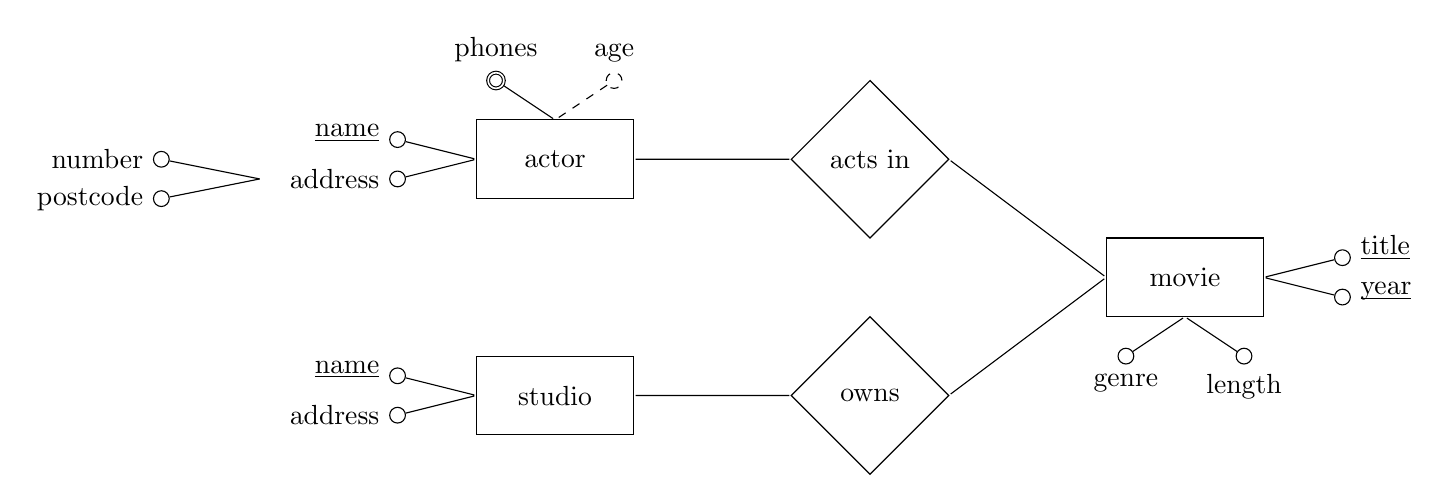
\begin{tikzpicture}
                    \entity{actor}{0, 0}{actor}
                    \entity{studio}{0, -3}{studio}
                    \relationship{actsin}{4, 0}{acts in}
                    \relationship{owns}{4, -3}{owns}
                    \entity{movie}{8, -1.5}{movie}
                    \nattribute{nactor}{-2, 0.25}{left}{\ulsmash{name}}
                    \nattribute{aactor}{-2, -0.25}{left}{address}
                    \mattribute{phones}{-0.75, 1}{above}{phones}
                    \dattribute{age}{0.75, 1}{above}{age}
                    \nattribute{nstudio}{-2, -2.75}{left}{\ulsmash{name}}
                    \nattribute{astudio}{-2, -3.25}{left}{address}
                    \nattribute{mtitle}{10, -1.25}{right}{\ulsmash{title}}
                    \nattribute{myear}{10, -1.75}{right}{\ulsmash{year}}
                    \nattribute{mgenre}{7.25, -2.5}{below}{genre}
                    \nattribute{mlength}{8.75, -2.5}{below}{length}
                    \nattribute{anumber}{-5, 0}{left}{number}
                    \nattribute{apostcode}{-5, -0.5}{left}{postcode}
                    \draw
                    (nactor) -- (actor-l)
                    (aactor) -- (actor-l)
                    (phones) -- (actor-u)
                    (age) edge[dashed] (actor-u)
                    (nstudio) -- (studio-l)
                    (astudio) -- (studio-l)
                    (actor-r) -- (actsin-l)
                    (studio-r) -- (owns-l)
                    (actsin-r) -- (movie-l)
                    (owns-r) -- (movie-l)
                    (movie-r) -- (mtitle)
                    (movie-r) -- (myear)
                    (movie-d) -- (mgenre)
                    (movie-d) -- (mlength)
                    (anumber) -- (-3.75, -0.25)
                    (apostcode) -- (-3.75, -0.25);
                \end{tikzpicture}
            \end{center}
            \subsubsection*{Cardinality Constraints}
                A relationship between two entity sets can be seen as one of the following (using the car example, where a person can drive $N$ cars, and a car can be driven by $M$ people);
                \begin{itemize}
                    \itemsep0em
                    \item one-to-one \hfill $M = 1, N = 1$
                    \item one-to-many \hfill $M = 1$
                    \item many-to-many \hfill no restrictions
                \end{itemize}
                \begin{center}
                    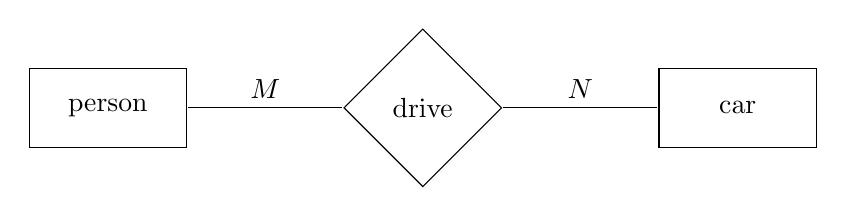
\begin{tikzpicture}
                        \entity{p}{0, 0}{person}
                        \relationship{d}{4, 0}{drive}
                        \entity{c}{8, 0}{car}
                        \draw
                        (p-r) edge[above] node{$M$} (d-l)
                        (d-r) edge[above] node{$N$} (c-l);
                    \end{tikzpicture}
                \end{center}
            \subsubsection*{Participation}
                Using the same example, we can force participation, which means that all entities must participate in a relationship, with a double line. The example below, with the cars, suggests that everyone drives at least 1 car, and car can have at most 1 driver (note that it doesn't mean that every car has a driver).
                \begin{center}
                    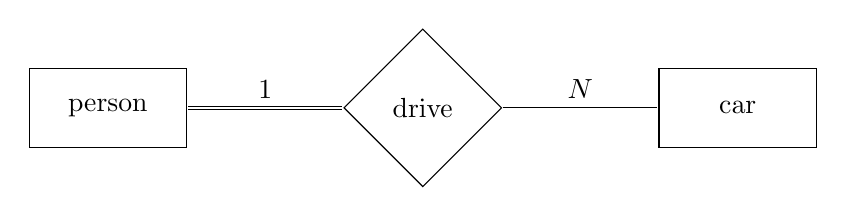
\begin{tikzpicture}
                        \entity{p}{0, 0}{person}
                        \relationship{d}{4, 0}{drive}
                        \entity{c}{8, 0}{car}
                        \draw
                        (p-r) edge[double, above] node{1} (d-l)
                        (d-r) edge[above] node{$N$} (c-l);
                    \end{tikzpicture}
                \end{center}
                Sometimes, instead of using double lines, E-R notation may allow explicit bounds. The below diagram suggests that staff work in exactly 1 branch, and that each branch must have at least 3 members of staff;
                \begin{center}
                    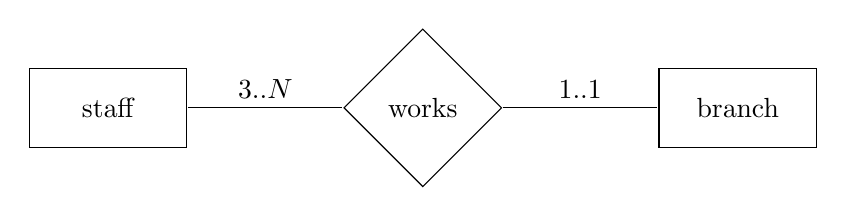
\begin{tikzpicture}
                        \entity{p}{0, 0}{staff}
                        \relationship{d}{4, 0}{works}
                        \entity{c}{8, 0}{branch}
                        \draw
                        (p-r) edge[above] node{$3..N$} (d-l)
                        (d-r) edge[above] node{$1..1$} (c-l);
                    \end{tikzpicture}
                \end{center}
            \subsubsection*{Fan, and Chasm Traps}
                See the diagrams in \textit{ER Modelling.pdf} for examples.
                \medskip

                We need to ensure that we do not allow ambiguous paths between entities. For example, if we say ~staff~ works for ~faculty~ which operates ~department~, if some member of staff works for Engineering, which operates both Computing, and EE, we can't follow a path from the staff member to their department. This can be solved by having the staff work for the department, which is operated by some faculty.
                \medskip

                If we can't follow a path between two entities, we may need to add another relation between them to specify the relationship.
            \subsubsection*{Weak Entities}
                Entities which cannot be uniquely identified by their own attributes are called \textbf{weak} entities, in contrast to \textbf{strong} entities which have primary keys. A weak entity has to be defined by a string entity. Weak entities are drawn as a double rectangle, and the relationship to the strong entity is drawn as a double diamond. The key for a weak entity is formed by combining the primary key of the strong entity with attributes of the weak entity (denoted by a dashed underline). For example, a room in a building is a \textbf{weak} entity, with a room number, and can be uniquely identified with the name of the building combined with the room number.
        \subsection*{ER to RM}
            Keys are used to join information when we do queries. The primary key is the unique identifier of a tuple, and a foreign key is the primary key of \textbf{another} table.
            \medskip

            Once we have an Entity Relationship Model, we can then map it to a relational schema. The schemas can then be refined with functional dependencies, and implemented with relational languages. A high level data model isn't the only concern for database design (considered a simpler aspect).
            \medskip

            If we consider a strong entity set, with simple attributes, we can easily create a table from it (see the example, ~movie~, drawn above).
            \begin{lstlisting}
                -- movie($\ulsmash{~title~}$, $\ulsmash{~year~}$, length, genre)

                CREATE TABLE movie (
                    title VARCHAR(120),
                    year INT,
                    length INT,
                    genre CHAR(20),

                    PRIMARY KEY (title, year)
                )
            \end{lstlisting}
            Composite attributes are also fairly easy to represent, since we just flatten it, therefore store each of the sub-attributes as their own field - consider the actor example (note that if the primary key is composite, we mark all the sub-attributes as primary keys). This example also shows how multi-valued attributes are stored - we create their own relation, and link back to the entity set with a foreign key constraint;
            \begin{lstlisting}
                -- actor($\ulsmash{~name~}$, number, postcode)
                -- actor_phones($\ulsmash{~actorName~}$, $\ulsmash{~phoneID~}$, $\textit{~other attributes~}$)

                CREATE TABLE actor (
                    name VARCHAR(60),
                    number INT,
                    postcode VARCHAR(10),
                    PRIMARY KEY (name)
                )

                CREATE TABLE actor_phones (
                    actorName VARCHAR(60),
                    phoneID VARCHAR(10),
                    ...
                    PRIMARY KEY (actorName, phoneID),
                    FOREIGN KEY (actorName) REFERENCES actor.name
                )
            \end{lstlisting}
            The relational model doesn't allow us to specify derived attributes, and we're therefore expected to calculate them with queries.
            \medskip

            We can also consider how many-to-many relationships can be represented (using the car example again). The first example is when a car can be driven by many people, and a person can drive many cars;
            \begin{lstlisting}
                -- person($\ulsmash{~ID~}$, $\textit{~other attributes~}$)
                -- car($\ulsmash{~regno~}$, $\textit{~other attributes~}$)
                -- drive($\ulsmash{~personID~}$, $\ulsmash{~regno~}$, $\textit{~other attributes~}$)

                CREATE TABLE drive (
                    personID VARCHAR(10),
                    regno VARCHAR(12),
                    ...
                    PRIMARY KEY (personID, regno),
                    FOREIGN KEY (personID) REFERENCES person.ID ON DELETE CASCADE,
                    FOREIGN KEY (regno) REFERENCES car.regno ON DELETE CASCADE
                )
            \end{lstlisting}
            However, it's easier to represent a one-to-many relationship, as we can simply include the primary key of the "one" relation as a foreign key in the many (where a car can be driven by 1 person, and a person can drive many cars). The representation for a one-to-one is similar, but the foreign key can be in either one, which is up to the designer;
            \begin{lstlisting}
                -- person($\ulsmash{~ID~}$, $\textit{~other attributes~}$)
                -- car($\ulsmash{~regno~}$, personID, $\textit{~other attributes~}$)

                CREATE TABLE car (
                    regno VARCHAR(12),
                    personID VARCHAR(10),
                    ...
                    PRIMARY KEY (regno),
                    FOREIGN KEY (personID) REFERENCES person.ID
                )
            \end{lstlisting}
            In a weak entity, we include the primary key of the strong relation as a foreign key, but also use it as part of the composite primary key for the weak entity. A delete cascade is also used, and finally the we use ~not null~ to ensure total participation;
            \begin{lstlisting}
                -- building($\ulsmash{~name~}$, $\textit{~other attributes~}$)
                -- room($\ulsmash{~no~}$, $\ulsmash{~buildingname~}$, $\textit{~other attributes~}$)

                CREATE TABLE room (
                    no VARCHAR(120),
                    buildingname VARCHAR(50) NOT NULL,
                    ...
                    PRIMARY KEY (no, buildingname),
                    FOREIGN KEY (buildingname) REFERENCES building.name ON DELETE CASCADE
                )
            \end{lstlisting}
            A multiway relationship can be mapped as several binary relationships, or we can generalise it to have the primary key consist of the relationship be composed of the primary keys of the many entity sets, and have the primary keys of the one entities be attributes. For roles, we map each role as a foreign key attribute in the entity set;
            \begin{lstlisting}
                -- movie($\ulsmash{~ID~}$, $\textit{~other attributes~}$)
                -- sequelof($\ulsmash{~originalID~}$, $\ulsmash{~sequelID~}$, $\textit{~other attributes~}$)

                CREATE TABLE sequelof (
                    originalID INT,
                    sequelID int,
                    ...
                    PRIMARY KEY (orignalID, sequelID),
                    FOREIGN KEY originalID REFERENCES movie.ID,
                    FOREIGN KEY sequelID REFERENCES movie.ID
                )
            \end{lstlisting}
            \subsubsection*{Extended Models}
                Newer models extend the classic model by supporting features from \textbf{object-oriented design}. We can look at how E-R models handle specialisation, or generalisation with \textbf{is-a hierarchies}. For example, we can specify that a ~cartoon~ \textbf{is-a} ~movie~, which means that it inherits all the attributes of movie, but can have more attributes. and relations. Once this extends on multiple levels, we begin to form a hierarchy.
        \subsection*{Relational Algebra}
            We can use \textbf{relational algebra} to construct new relations from existing ones, the operators include selection, projection, intersection, union, difference, and product. Consider the examples below, ~a~, ~b~, and ~c~ are all integers. Intersection, union, and difference will be omitted, since those are fairly self-explanatory.
            \begin{center}
                \begin{tabular}{|cccccc|ccc|ccc|ccc|}
                    \hline
                    \multicolumn{6}{|c|}{$R$} & \multicolumn{3}{c|}{$\pi_{~a,c,e~}(R)$} & \multicolumn{3}{c|}{$S$} & \multicolumn{3}{c|}{$\sigma_{~a>3|b<5~}(S)$} \\
                    \hline
                    ~a~ & ~b~ & ~c~ & ~d~ & ~e~ & ~f~ & ~a~ & ~c~ & ~e~ & ~a~ & ~b~ & ~c~ & ~a~ & ~b~ & ~c~ \\
                    \hline
                    1 & 2 & 3 & 4 & 5 & 6 & 1 & 3 & 5 & 3 & 2 & 3 & 3 & 2 & 3 \\
                    1 & 1 & 1 & 1 & 1 & 1 & 1 & 1 & 1 & 2 & 1 & 7 & 8 & 2 & 2 \\
                    2 & 2 & 2 & 2 & 2 & 2 & 2 & 2 & 2 & 8 & 2 & 2 & & & \\
                    1 & 2 & 3 & 4 & 5 & 8 & & & & 1 & 2 & 9 & & & \\
                    \hline
                \end{tabular}
            \end{center}
            The syntax in use here for projection is $\pi_{~attributes~}(T)$, and likewise for selection it's $\sigma_{~condition~}(T)$. The former returns a relation with only the listed attributes, and the only takes rows which satisfy the given condition. Neither will return duplicate rows. Here is an example of a Cartesian product;
            \begin{center}
                \begin{tabular}{|cc|ccc|ccccc|}
                    \hline
                    \multicolumn{2}{|c|}{$R$} & \multicolumn{3}{c|}{$S$} & \multicolumn{5}{c|}{$R \times S$} \\
                    \hline
                    ~a~ & ~b~ & ~c~ & ~d~ & ~e~ & ~a~ & ~b~ & ~c~ & ~d~ & ~e~ \\
                    \hline
                    1 & 2 & 1 & 2 & 3 & 1 & 2 & 1 & 2 & 3 \\
                    3 & 4 & 4 & 5 & 6 & 1 & 2 & 4 & 5 & 6 \\
                    & & 7 & 8 & 9 & 1 & 2 & 7 & 8 & 9 \\
                    & & & & & 3 & 4 & 1 & 2 & 3 \\
                    & & & & & 3 & 4 & 4 & 5 & 6 \\
                    & & & & & 3 & 4 & 7 & 8 & 9 \\
                    \hline
                \end{tabular}
            \end{center}
            We can take a natural join, where the resulting relation contains all the tuples that have matching attributes in $R$, and $S$. This is less common, and we'd typically use something closer to $R \bowtie_{R.~b~ = S.~b~} S$. Note that in this case, they are the same, since that's the only attribute that overlaps;
            \begin{center}
                \begin{tabular}{|cc|ccc|cccc|}
                    \hline
                    \multicolumn{2}{|c|}{$R$} & \multicolumn{3}{c|}{$S$} & \multicolumn{4}{c|}{$R \bowtie S$} \\
                    \hline
                    ~a~ & ~b~ & ~b~ & ~c~ & ~d~ & ~a~ & ~b~ & ~c~ & ~d~ \\
                    \hline
                    1 & 2 & 1 & 2 & 3 & 1 & 2 & 5 & 6 \\
                    1 & 3 & 2 & 5 & 6 & 3 & 4 & 8 & 9 \\
                    3 & 4 & 4 & 8 & 9 & 3 & 4 & 9 & 9 \\
                    & & 4 & 9 & 9 & & & & \\
                    \hline
                \end{tabular}
            \end{center}
            Attributes can also be renamed with the notation $\rho_{~new/old~, ...}(R)$ notation, which is fairly self-explanatory.
        \subsection*{Functional Dependencies}
            Relational database schemas should be normalised, which helps reduce redundancy, and avoids update, and deletion anomalies. The basis for normalisation is the concept of \textbf{functional dependency}, and \textbf{keys}. Consider the following example, which can experience update anomalies;
            \begin{center}
                \begin{tabular}{|l|l|l|l|l|}
                    \hline
                    producer & city & product no. & price & quantity \\
                    \hline
                    \hline
                    3 & London & 52 & 65 & 4 \\
                    22 & Birmingham & 10 & 15 & 5 \\
                    22 & Birmingham & 12 & 4 & 11 \\
                    3 & London & 44 & 43 & 32 \\
                    3 & London & 43 & 3 & 27 \\
                    \hline
                \end{tabular}
            \end{center}
            If an existing producer changes address, and tuples aren't updated, then it leads to incoherence (as the data would now be invalid). If a new tuple / row is inserted, and the producer already exists, but with an older address, we will once again have incoherence. If a producer doesn't have any open orders, say rows 1, and 5 didn't exist, then data about producer 3 would be lost. The price of the product doesn't depend on the producer, and the location of the producer doesn't have anything to do with the product. There is also redundant data, since the address is duplicated. Ideally, the data should be stored like this;
            \begin{center}
                \begin{minipage}[t]{0.4\textwidth}
                    \begin{tabular}{|l|l|l|}
                        \hline
                        \multicolumn{3}{|l|}{Open Orders} \\
                        \hline
                        producer no. & product no. & quantity \\
                        \hline
                        \hline
                        3 & 52 & 4 \\
                        22 & 10 & 5 \\
                        22 & 12 & 11 \\
                        3 & 44 & 32 \\
                        3 & 43 & 27 \\
                        \hline
                    \end{tabular}
                \end{minipage}
                \begin{minipage}[t]{0.3\textwidth}
                    \begin{tabular}{|l|l|}
                        \hline
                        \multicolumn{2}{|l|}{Producer} \\
                        \hline
                        producer no. & city \\
                        \hline
                        \hline
                        3 & London \\
                        22 & Birmingham \\
                        & \\
                        & \\
                        & \\
                        \hline
                    \end{tabular}
                \end{minipage}
                \begin{minipage}[t]{0.21\textwidth}
                    \begin{tabular}{|l|l|}
                        \hline
                        \multicolumn{2}{|l|}{Product} \\
                        \hline
                        product no. & price \\
                        \hline
                        \hline
                        52 & 65 \\
                        10 & 15 \\
                        12 & 4 \\
                        44 & 43 \\
                        43 & 3 \\
                        \hline
                    \end{tabular}
                \end{minipage}
            \end{center}
            A functional dependency is a constraint that if two tuples of a relation $R$ agree on a set of attributes $A_1, A_2, ..., A_n$, then they must also agree on the set of attributes $B_1, B_2, ..., B_m$. This can be written as $A_1, A_2, ..., A_n \rightarrow B_1, B_2, ..., B_m$, and therefore the $B$ set is functionally dependant on the $A$ set, or the $A$ set functionally determines the $B$ set. Therefore, for any set of values $A$, then there is only one set of values $B$. The normal forms a designer can use are defined in terms of their functional dependencies. This can be summarised by the following examples;
            \begin{center}
                \begin{tabular}{|c|c|c|}
                    \hline
                    functional dependency & for all tuple pairs, $x$, $y$, if & then assert \\
                    \hline
                    $A \rightarrow K$ & $x.A = y.A$ & $x.K = y.K$ \\
                    \hline
                    $A, B \rightarrow K$ & $x.A = y.A$ & $x.K = y.K$ \\
                    & $x.B = y.B$ & \\
                    \hline
                    $A \rightarrow K, L$ & $x.A = y.A$ & $x.K = y.K$ \\
                    & & $x.L = y.L$ \\
                    \hline
                    $A, B \rightarrow K, L$ & $x.A = y.A$ & $x.K = y.K$ \\
                    & $x.B = y.B$ & $x.L = y.L$ \\
                    \hline
                \end{tabular}
            \end{center}
            Note that if we have two functional dependencies, $A, B \rightarrow K$, and $A, B \rightarrow L$, it's trivial to combine them as $A, B \rightarrow K, L$ (or to split them). If we have the functional dependency $A, B, C, D, E \rightarrow A, C, X, Y, Z$, we can remove all the attributes on the right hand side, that are on the left hand side, such that the aforementioned FD reduces to $A, B, C, D, E \rightarrow X, Y, Z$. A \textbf{trivial} FD is one where all the attributes on the RHS are on the LHS.
            \subsubsection*{Keys}
                If we have some set of attributes $A_1, A_2, ..., A_n$, functionally determine all the remaining attributes of the relation, then the set $A$ is a \textbf{superkey}. This also implies that two tuples cannot have the same superkey values, due to the uniqueness property. Let there be a set of all attributes in the relation, $K$, and the superkey set $S$. Therefore we can state $S \rightarrow \{ x \in K\ |\ x \notin S \}$. A single relation may have more than one superkey, and superkeys can contain attributes that aren't strictly required. Generally, we are interested in superkeys where there isn't a subset of the superkey (hence the smallest superkey, by the irreducibility property), and this minimal superkey is referred to as the \textbf{candidate key}. If we have more than one candidate key, we can choose one of them to act as the primary key. A candidate key is also often referred to as just a \textbf{key}.
            \subsubsection*{Closure}
                The set of all attributes functionally determined by a set $L$, under a set of dependencies $F$, the closure of $L$, denoted as $L^+$. If $L^+$ contains all the attributes of $R$, then it follows that $L$ is a superkey of $R$. If $\text{RHS} \subseteq \text{LHS}^+$, then $\text{LHS} \rightarrow \text{RHS}$ holds.
                \medskip

                In order to compute the closure of a set of attributes, $L$, under a set of FDs given in the form $\text{LHS} \rightarrow \text{RHS}$, we keep adding all the LHSs which exist as a subset of $L$, and add the RHS to $L$. We repeat this until we can no longer add anymore RHSs. The final value is referred to as $L^+$. Given the starting value of $L = \{A, B\}$, and the following FD set;
                \begin{enumerate}[(1)]
                    \itemsep0em
                    \item $A, B \rightarrow C$
                    \item $B, C \rightarrow A, D$
                    \item $D \rightarrow E$
                    \item $C, F \rightarrow B$
                \end{enumerate}
                Starting with (1), both $A$, and $B$ are in $L$, so we can add $C$. Now that $C$ is in $L$, and $B$ was already there, we can add $D$ (no need to add $A$) from (2). Since we have $D$ in $L$, we can add $E$. There is nothing else we can do, since $F$ is not in $L$. Hence the value of $L^+ = \{A, B, C, D, E\}$.
            \subsubsection*{Armstrong's Axioms}
                This is a sound (doesn't generate incorrect FDs), and compete (allows us to derive all valid FDs) axiomisation of FDs. Given attributes $A, B, C, ...$, and sets of attributes $\alpha, \beta, \gamma$, we have the following axioms;
                \begin{itemize}
                    \itemsep0em
                    \item reflexivity (trivial FDs) \hfill $\alpha \rightarrow \beta$ always holds if $\beta \subseteq \alpha$
                    \item augmentation \hfill if $\alpha \rightarrow \beta$, then it follows $\alpha \gamma \rightarrow \beta \gamma$
                    \item transitivity \hfill if $\alpha \rightarrow \beta$, and $\beta \rightarrow \gamma$, then $\alpha \rightarrow \gamma$
                    \item (derived) union \hfill if $\alpha \rightarrow \beta$, and $\alpha \rightarrow \gamma$, then $\alpha \rightarrow \beta \gamma$
                    \item (derived) decomposition \hfill if $\alpha \rightarrow \beta \gamma$, then $\alpha \rightarrow \beta$, and $\alpha \rightarrow \gamma$
                    \item (derived) pseudotransitivity \hfill if $\alpha \rightarrow \beta$, and $\delta \beta \rightarrow \gamma$, then $\delta \alpha \rightarrow \gamma$
                \end{itemize}
            \subsubsection*{Closure, and Covers}
                Similar to attributes, we can find the closure of a FD set, which is the set of all FDs that can be inferred, denoted as $F^+$. This can be approached by applying Armstrong's axioms. We start by initialising $F^+$ to the set $F$. By applying reflexivity, and augmentation, we can add new FDs to $F^+$. Transitivity can then be applied to suitable FDs, and adding the derived ones to $F^+$. This is repeated until no more changes occur.
                \medskip

                We can say two FD sets $F_1$, and $F_2$ are equivalent if they each imply the other - if any relation instance satisfying $F_1$ also satisfies $F_2$, they are said to be covers of each other. A cover is canonical / minimal / irreducible if each LHS is unique, and no FD can be deleted from the cover, and still maintain an equivalent FD set. Additionally, no attributes can be deleted from any FD set, and still have an equivalent set. Therefore, the canonical cover has no redundant dependencies, nor attributes.
                \medskip

                The method for testing whether some attribute, $X$, is extraneous depends on whether it's on the LHS, or RHS. For an attribute $X$ on the LHS, we can say $X$ is extraneous if $\text{RHS} \subseteq \{\text{LHS} - X\}^+$ under the FD set - note that here we are referring to closure on attributes, not FDs. On the other hand (no pun intended, I'm so depressed), an attribute $X$ on the RHS is extraneous if $X \in \text{LHS}^+$ under the FD set, where $X$ is removed from the RHS of the FD.
                \medskip

                To compute a canonical cover $F$ for an FD set, we can use the following algorithm;
                \begin{lstlisting}
                    let $F$ := FD set
                    do
                        replace dependencies of $\alpha \rightarrow \beta$ and $\alpha \rightarrow \gamma$, with $\alpha \rightarrow \beta \gamma$
                        remove all extraneous attributes one at a time
                    until $F$ doesn't change
                \end{lstlisting}
        \subsection*{Normalisation}
            As previously mentioned, in the previous section, normalisation reduces data duplication, and anomalies. One of the approaches taken to develop a normalised schema is to start with a few big relations, and then decompose them into a suitable normal form. The ones we'll look at are \textbf{Boyce-Codd Normal Form (BCNF)}, and \textbf{Third Normal Form (3NF)}. Consider the following example, which is just a "big" relation;
            \begin{center}
                \begin{tabular}{|c|c|c|c|c|c|}
                    \hline
                    ~title~ & ~year~ & ~length~ & ~genre~ & ~studio~ & ~actor~ \\
                    \hline
                    \hline
                    Star Wars & 1977 & 124 & Science Fiction & Fox & Carrie Fisher \\
                    \hline
                    Star Wars & 1977 & 124 & Science Fiction & Fox & Mark Hamill \\
                    \hline
                    Star Wars & 1977 & 124 & Science Fiction & Fox & Harrison Ford \\
                    \hline
                    Gone with the Wind & 1939 & 231 & Drama & MGM & Vivien Leigh \\
                    \hline
                    Luis' World & 1992 & 95 & Comedy & Paramount & Dana Carvey \\
                    \hline
                    Luis' World & 1992 & 95 & Comedy & Paramount & Mile Myers \\
                    \hline
                \end{tabular}
            \end{center}
            You'll notice straight away that there is a huge amount of redundant, repeated data, which is present in multiple rows. Updating the ~length~ of Star Wars would require 3 updates (for the relation to remain consistent), which is error prone. Inserting a new actor for a movie would require duplicating a fair bit of data, and would require checks to maintain consistency. Finally, deleting Vivien Leigh would delete the entire row, which deletes information about the movie.
            \subsubsection*{Decomposition}
                Given a relation $R(A_1, A_2, ..., A_n)$, we can decompose it into two projected relations $S$, and $T$, such that $\text{attr}(R) = \text{attr}(S) \cup \text{attr}(T)$. This also means that $S = \pi_{\text{attr}(S)}(R)$, and similar for $T$.
                \medskip

                When we decompose a relation, it's crucial for us to ensure we can recover the original relation by joining the decomposed relations, and also preserve the FDs of the original relation. Note that the latter isn't always possible with BCNF.
                \medskip

                Given $R$ decomposed into $S$, and $T$, the decomposition is \textbf{lossless} if at least one of the following FDs hold in the closure of the FD set of $R$;
                \begin{itemize}
                    \itemsep0em
                    \item $\text{attr}(S) \cap \text{attr}(T) \rightarrow \text{attr}(S)$
                    \item $\text{attr}(S) \cap \text{attr}(T) \rightarrow \text{attr}(T)$
                    \item this means the common attributes of $S$, and $T$ form a superkey of either of the decomposed relations
                \end{itemize}
                If we're able to check the FDs of $R$ without joining the decomposed sets, then the decomposition is \textbf{dependency preserving}.
                \medskip

                Consider the following example, on $R(A, B, C)$, with the FD set $\{A \rightarrow B, B \rightarrow C\}$;
                \begin{center}
                    \vspace{-\baselineskip}
                    \begin{tabularx}{\textwidth}{|l|l|X|}
                        \hline
                        decomposition & lossless? & dependency preserving? \\
                        \hline
                        $S(A, B)$ & $B \rightarrow A, B$ doesn't hold & yes, $A \rightarrow B$ is checked with $S$, and $B \rightarrow C$ with $T$ \\
                        $T(B, C)$ & $B \rightarrow B, C$ holds $\therefore$ lossless & \\
                        \hline
                        $S(A, B)$ & $A \rightarrow A, B$ holds $\therefore$ lossless & no, $B \rightarrow C$ cannot be checked without joining \\
                        $T(A, C)$ & $A \rightarrow A, C$ holds also & \\
                        \hline
                    \end{tabularx}
                    \vspace{-2\baselineskip}
                \end{center}
            \subsubsection*{Boyce-Codd Normal Form}
                \textbf{A relation $R$ is in BCNF, if and only if, for all non-trivial FDs (including derived FDs) of the relation, the LHS of every FD is a superkey (i.e. contains a key)}
                \bigskip

                For example, if we have the FD $~title~, ~year~ \rightarrow ~length~, ~genre~, ~studio~$, it's not in BCNF, as ~title~, ~year~ doesn't functionally determine ~actor~.
                \medskip

                In order to convert something into BCNF, we first initialise a set of relations with just $R$. While the set contains relations that violate the rules of BCNF, take one of them, let it be $V$. Let us take some non-trivial FD for $V$, of the form $\text{LHS} \rightarrow \text{RHS}$; fulfilling the conditions $\text{LHS} \cap \text{RHS} = \emptyset$ (therefore we may need to check a derived FD for decomposed relations), and $\text{LHS} \rightarrow \text{attr}(V)$ does not hold for the FD$^+$ of $R$ (therefore, LHS is not a superkey of $R$). Now remove $V$ from the set of relations. Add a new relation $R_k(\text{LHS} \cup \text{RHS})$, and another relation $R_l(\text{attr}(V) - \text{RHS})$ to the set of decompositions. This process is then recursively applied to the child relations. Consider the following example;
                \medskip

                $R(A, B, C, D, E, F, G, H, I, J, K)$, and the following FDs;
                \begin{itemize}
                    \itemsep0em
                    \item $A \rightarrow B, C, D$
                    \item $H, I \rightarrow J$
                    \item $A, E, F, G \rightarrow H, I, K$
                \end{itemize}
                \begin{center}
                    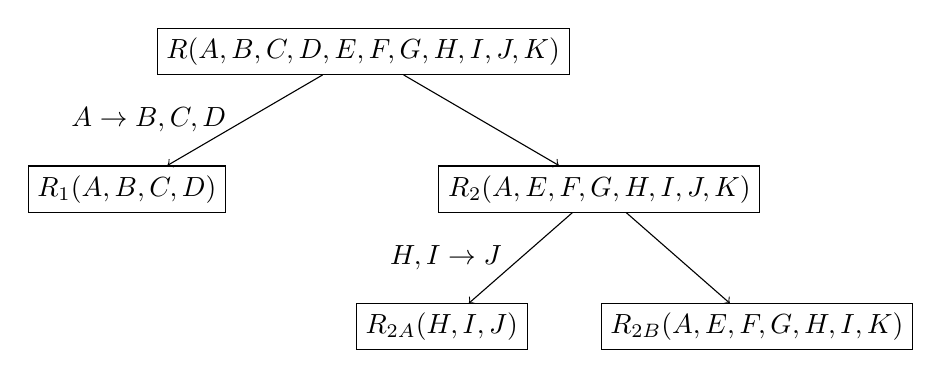
\begin{tikzpicture}
                        \node[draw] (o) at (0, 0) {$R(A, B, C, D, E, F, G, H, I, J, K)$};
                        \node[draw] (ol) at (-3, -1.75) {$R_1(A, B, C, D)$};
                        \node[draw] (or) at (3, -1.75) {$R_2(A, E, F, G, H, I, J, K)$};
                        \node[draw] (orl) at (1, -3.5) {$R_{2A}(H, I, J)$};
                        \node[draw] (orr) at (5, -3.5) {$R_{2B}(A, E, F, G, H, I, K)$};
                        \draw
                        (o) edge[->, left] node{$A \rightarrow B, C, D\ $} (ol)
                        (o) edge[->] (or)
                        (or) edge[->, left] node{$H, I \rightarrow J\ $} (orl)
                        (or) edge[->] (orr);
                    \end{tikzpicture}
                \end{center}
                Honestly, just practice this.
            \subsubsection*{Recovering Data}
                When we decompose into BCNF, it's crucial that we're able to recover the original relation by joining the decomposed ones. As long as the FDs hold for the original relation, it will always be possible. However; if the FDs don't hold, we'd end up with false data; as the join would generate tuples that don't exist in the original relation.
            \subsubsection*{Dependency Preservation}
                As previously mentioned, we know that BCNF doesn't always preserve dependencies, which can be shown here. Let there be a relation $R(A, B, C)$, and the FD set; $\{\{A, B\} \rightarrow C, C \rightarrow B\}$. We wouldn't be able to check $A, B \rightarrow C$ without the RDBMS joining the relations.
                \begin{center}
                    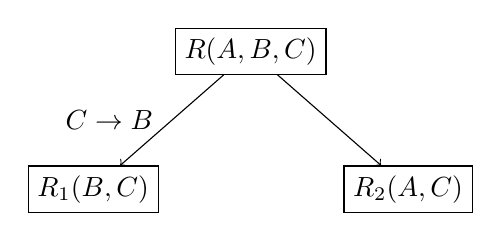
\begin{tikzpicture}
                        \node[draw] (o) at (0, 0) {$R(A, B, C)$};
                        \node[draw] (ol) at (-2, -1.75) {$R_1(B, C)$};
                        \node[draw] (or) at (2, -1.75) {$R_2(A, C)$};
                        \draw
                        (o) edge[->, left] node{$C \rightarrow B\ $} (ol)
                        (o) edge[->] (or);
                    \end{tikzpicture}
                \end{center}
            \subsubsection*{Third Normal Form}
                \textbf{A relation $R$ is in 3NF, if and only if, the LHS of every nontrivial FD is a superkey (same as BCNF test), or if every attribute on the RHS of a FD is prime (if it is a member of any key of the relation)}
                \bigskip

                When a BCNF decomposition doesn't preserve the original FDs, we can either "live with" the violating dependencies, or use a weaker normal form which preserves FDs, but has redundancy. With \textbf{3NF}, there always exists a dependency preserving, lossless decomposition.
                \medskip

                In order to decompose a relation $R$, and a set of FDs $F$ for $R$, we can generate a set of decomposed relations $D$. We first need to find $C$, a canonical cover for $F$, such that it's a minimal FD set for $R$. Initialise $D$ to be $\emptyset$. For every canonical FD, in the form $\text{LHS} \rightarrow \text{RHS}$, we add a new relation $(\text{LHS} \cup \text{RHS})$ to $D$. Now, for every relation in $D$, if it is a subset of another relation in $D$, we remove it. Finally, if none of the relations in $D$ include a key for $R$, we add a new relation to $D$, which contains a key.
                \medskip

                Consider the following relation $R(A, B, C, D, E, F, G, H, I)$, a set of keys $\{\{A, B\}, \{A, D\}, \{B, D\}\}$ with the following FD set (and its canonical cover on the right);
                \begin{itemize}
                    \itemsep0em
                    \item $A, B \rightarrow D, E$ \hfill $A, B \rightarrow D$
                    \item $A \rightarrow I$ \hfill $A \rightarrow I$
                    \item $B \rightarrow C, F, G, H$ \hfill $B \rightarrow C, F, G$
                    \item $G \rightarrow H$ \hfill $G \rightarrow H$
                    \item $A, D \rightarrow B, C, E, F, G, H$ \hfill $A, D \rightarrow B$
                    \item $B, D \rightarrow A, I, E$ \hfill $B, D \rightarrow A, E$
                \end{itemize}
                \begin{center}
                    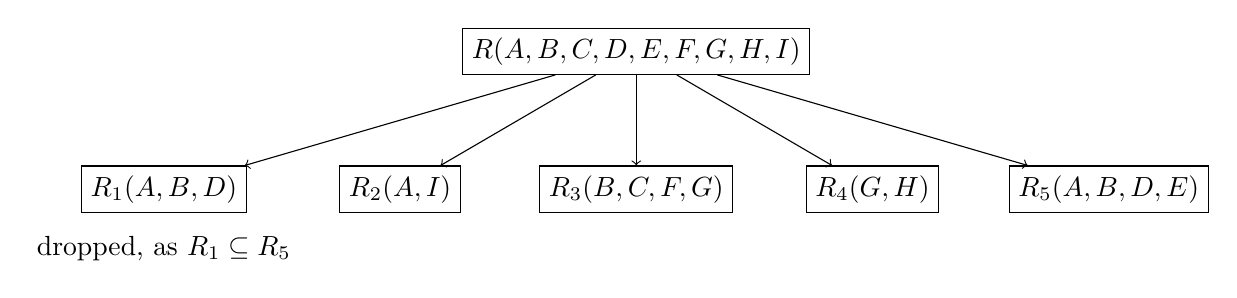
\begin{tikzpicture}
                        \node[draw] (r) at (0, 0) {$R(A, B, C, D, E, F, G, H, I)$};
                        \node[draw] (r1) at (-6, -1.75) {$R_1(A, B, D)$};
                        \node[draw] (r2) at (-3, -1.75) {$R_2(A, I)$};
                        \node[draw] (r3) at (0, -1.75) {$R_3(B, C, F, G)$};
                        \node[draw] (r4) at (3, -1.75) {$R_4(G, H)$};
                        \node[draw] (r5) at (6, -1.75) {$R_5(A, B, D, E)$};
                        \node[] () at (-6, -2.5) {dropped, as $R_1 \subseteq R_5$};
                        \draw
                        (r) edge[->] (r1)
                        (r) edge[->] (r2)
                        (r) edge[->] (r3)
                        (r) edge[->] (r4)
                        (r) edge[->] (r5);
                    \end{tikzpicture}
                \end{center}
        \subsection*{SQL}
            \textbf{Structured Query Language} is the most common language for relational databases, with use in more than 99\% of applications. It supports schema creation, modification, data insertion, retrieval, updates, deletion, and a lot more. Translating from the relational algebra we previously done, to SQL, can be done with the table below;
            \begin{center}
                \begin{tabularx}{\textwidth}{|c|c|X|}
                    \hline
                    relational algebra & SQL & comments\\
                    \hline
                    \hline
                    $R \cup S$ & $R ~ UNION ~ S$ & \\
                    $R \cap S$ & $R ~ INTERSECT ~ S$ & \\
                    $R - S$ & $R ~ EXCEPT ~ S$ & \\
                    $\pi_~attributes~(R)$ & $~SELECT attributes FROM ~ R$ & \\
                    $\sigma_~condition~(R)$ & $~FROM ~ R ~ WHERE condition~$ & \\
                    $R \times S$ & $R, S$ or $R ~ CROSS JOIN ~ S$ & \\
                    $R \bowtie S$ & $R ~ NATURAL JOIN ~ S$ & \\
                    $R \bowtie_~condition~ S$ & $R ~ JOIN ~ S ~  ON condition~$ & \\
                    relation & table & persistent relations stored on disk \\
                    relational expression & views & based on other relations, not normally stored \\
                    tuple & row & also called a record \\
                    attribute & column & also called a field \\
                    domain & type & includes ~char~, ~int~, ~float~, ~date~, ~time~, etc. \\
                    \hline
                \end{tabularx}
                \vspace{-2\baselineskip}
            \end{center}
            However, SQL differs from the theory we've studied so far, as it is based on multi-sets, and therefore can contain duplicate rows / tuples. It's still best practice to avoid them. Not all attributes need to be filled in, and therefore can be left ~null~, once again this should be avoided; because of this, booleans are three-valued (true, false, and unknown). Most implementations have a wide range of types, and therefore numbers have multiple types - arithmetic operators are usually available. Strings can either be a fixed length, and padded with spaces, or varying length. The concatenation operator used in SQL is ~||~, and we can use pattern matching, with ~\_~ denoting any character, and ~\%~ matching zero, or more characters. We can store bits, bytes, and large binary objects (blobs) to hold images, movies, and other files.
            \medskip

            With booleans, we have additional comparison operators such as ~BETWEEN~, ~NOT BETWEEN~, ~IN~, and ~NOT IN~, all of which should be fairly self-explanatory. The truth values for 3VL (three valued logic) can be computed with the following mapping;
            \begin{itemize}
                \itemsep0em
                \item 1 - true
                \item $\frac{1}{2}$ - unknown
                \item 0 - false
                \item $x$ ~AND~ $y$ = min($x, y$)
                \item $x$ ~OR~ $y$ = max($x, y$)
                \item ~NOT~ $x$ = $1 - x$
            \end{itemize}
            \medskip

            It's also important to remember that any arithmetic which uses a ~null~, will result in ~null~. Any comparisons that use ~null~ will result in unknown.
            \subsubsection*{Queries}
                In order to save space, all comments will be done inline, in the SQL code listing below;
                \begin{lstlisting}
                    -- movie(title, year, length, genre, studio, producer)
                    -- casting(title, year, name)

                    -- note that the results of a selection is still a relation, and therefore we can use it as a subquery in other expressions
                    SELECT title, length/60 AS hours -- projected attributes (and a rename)
                    FROM movie -- the relation
                    WHERE studio='fox' AND year > 1990 -- the condition
                    ORDER BY year DESC, title ASC -- sorts first by year
                    -- note that we're using attributes which aren't in the projection, the order of operations is FROM, WHERE, ORDER, SELECT
                    -- note that we can also prefix the fields, to make it more readable
                \end{lstlisting}
                In order to join two relations, we can use a ~JOIN~;
                \begin{lstlisting}
                    SELECT title, year, name
                    FROM movie JOIN casting ON (movie.producer=casting.name)
                    -- we can do a theta join with an ON, and a condition

                    SELECT title
                    FROM movie JOIN casting USING (title, year)
                    -- note that this is the same as ON (movie.title=casting.title AND movie.year=casting.year)

                    SELECT c1.name, c2.name
                    FROM casting AS c1 JOIN casting c2 -- note how we can omit AS for readability
                    ON c1.address = c2.address AND
                       c1.name < c2.name
                    -- we can do a self join, but we have to name the relation, these are called correlation names
                \end{lstlisting}
                We can also consider the different types of joins, either natural (by matching attributes), or theta (by condition);
                \begin{itemize}
                    \itemsep0em
                    \item inner join \hfill returns tuples when there is at least one match in both sides
                    \item left outer join (~LOJ~) \hfill similar to inner join, but will include all tuples from the left relation
                    \item right outer join (~ROJ~) \hfill similar to inner, but includes all tuples from the right relation
                    \item full outer join (~FOJ~) \hfill similar to inner, but includes all unmatched tuples
                \end{itemize}
                \begin{center}
                    \begin{tabular}{|c|c|c||c|c|c||c|c|c|c||c|c|c|c||c|c|c|c|}
                        \hline
                        \multicolumn{3}{|c||}{$L$} & \multicolumn{3}{c||}{$R$} & \multicolumn{4}{c||}{$L$ ~LOJ~ $R$} & \multicolumn{4}{c||}{$L$ ~ROJ~ $R$} & \multicolumn{4}{c|}{$L$ ~FOJ~ $R$} \\
                        \hline
                        ~a~ & ~b~ & ~c~ & ~a~ & ~b~ & ~d~ & ~a~ & ~b~ & ~c~ & ~d~ & ~a~ & ~b~ & ~c~ & ~d~ & ~a~ & ~b~ & ~c~ & ~d~ \\
                        \hline
                        \hline
                        1 & 2 & 3 & 2 & 3 & A & 1 & 2 & 3 & A & 1 & 2 & 3 & A & 1 & 2 & 3 & A \\
                        \hline
                        4 & 5 & 6 & 2 & 3 & B & 1 & 2 & 3 & B & 1 & 2 & 3 & B & 1 & 2 & 3 & B \\
                        \hline
                        7 & 8 & 9 & 6 & 8 & C & 4 & 5 & 6 & N & N & 6 & 8 & C & 4 & 5 & 6 & N \\
                        \hline
                        & & & & & & 7 & 8 & 9 & N & & & & & 7 & 8 & 9 & N \\
                        \hline
                        & & & & & & & & & & & & & & N & 6 & 8 & C \\
                        \hline
                    \end{tabular}
                \end{center}
                \begin{lstlisting}
                    SELECT DISTINCT title, year, name -- selects only unique tuples
                    FROM movie LEFT OUTER JOIN casting ON
                        movie.producer=casting.name AND movie.year=casting.year
                \end{lstlisting}
                We also have a set of aggregation functions, which can be used to calculate a single value, for example;
                \begin{lstlisting}
                    SELECT department
                           COUNT(*) as professors,
                           SUM(salary) as totalsalary,
                           AVG(salary) as averagesalary,
                           MIN(age) as youngest,
                           MAX(age) as oldest
                    FROM employee
                    WHERE position='Professor'
                    GROUP BY department
                    HAVING COUNT(*) >= 10
                    ORDER BY totalsalary DESC
                \end{lstlisting}
                This creates a tuple for each department; the results are then sorted in descending order by total salary. Any non-aggregates used in the projection, or the ~HAVING~ filter \textbf{must} be included in the ~GROUP BY~ list. Only departments with at least 10 professors are listed.
            \subsubsection*{Subqueries}
                A powerful feature of ~SELECT~s is that we can also use them as subqueries in expressions, by wrapping them in brackets. The types supported by SQL are;
                \begin{itemize}
                    \itemsep0em
                    \item scalar subquery
                        \subitem a subquery that produces a single value, normally uses an aggregate function
                        \begin{lstlisting}
                            SELECT title,
                                (SELECT count(name)
                                 FROM casting
                                 WHERE casting.title=movie.title) AS numactors
                            FROM movie
                            -- note how the outer query is related to the subquery; this is an example of a correlated subquery that has to be evaluated for each outer tuple

                            SELECT title, count(name) as numactors
                            FROM movie JOIN casting USING (title)
                            GROUP BY title
                            -- this is equivalent, and is clearer
                        \end{lstlisting}
                    \item set subquery
                        \subitem creates a set of distinct values (a single column), typically used for set membership with ~(NOT) IN~, or set comparisons with ~ALL~ or ~SOME~
                        \begin{lstlisting}
                            SELECT title
                            FROM movie
                            WHERE studio IN (SELECT name
                                             FROM studio
                                             WHERE address LIKE 'C%')
                            SELECT name
                            FROM casting
                            WHERE (title, year) NOT IN (SELECT title, year
                                                        FROM movie
                                                        WHERE genre='sf')
                            -- note how we're able to match on tuple values
                            SELECT title
                            FROM movie m1
                            WHERE year < SOME(SELECT year
                                              FROM movie m2
                                              WHERE m2.title=m1.title)
                            -- the keywords ALL, and SOME can be used with any comparator

                            SELECT name
                            FROM employee
                            WHERE salary <> ALL(SELECT salary
                                                FROM employee
                                                WHERE position='Professor'
                        \end{lstlisting}
                    \item relation subquery
                        \subitem produces a relation, which is typically used as an operand, used with operators ~(NOT) EXISTS~ to check if it's empty, or operators ~(NOT) UNIQUE~ to test for duplicate tuples
                        \begin{lstlisting}
                            SELECT title
                            FROM movie m1
                            WHERE NOT EXISTS(SELECT *
                                             FROM movie m2
                                             WHERE m2.title=m1.title AND m1.year<>m2.year)
                        \end{lstlisting}
                \end{itemize}
        \subsection*{SQL Data Definition}
            SQL's DDL is concerned with schema creation, as well as the specification of any constraints. This course mainly focuses on base relations (which are stored tables), and lightly touches on derived relations (views). The constraints we deal with in SQL include type, primary / foreign key constraints, uniqueness, checking a value exists (not null), check constraints, as well as assertions.
            \subsubsection*{Creating a Relation}
                Given some relation ~movie(\ulsmash{title}, \ulsmash{year}, length, genre, ISAN)~, the following SQL instruction will create the table;
                \begin{lstlisting}
                    CREATE TABLE movie (
                        title VARCHAR(120),
                        year INT DEFAULT 2011,
                        length INT NOT NULL DEFAULT 0,
                        genre CHAR(20) NOT NULL,
                        ISAN CHAR(24) NOT NULL,
                        PRIMARY KEY (title, year),
                        UNIQUE (ISAN)
                    )
                    -- this table can be deleted with 'DROP TABLE movie'
                    -- please sanitise your inputs (https://xkcd.com/327/)
                \end{lstlisting}
                We can then modify the schema, with the ~ALTER TABLE~ command, for example (leads to the modified schema ~movie(\ulsmash{title}, \ulsmash{year}, genre, studio, ISAN)~);
                \begin{lstlisting}
                    ALTER TABLE movie ADD studio CHAR(16) DEFAULT '';
                    ALTER TABLE movie DROP length;
                \end{lstlisting}
                Note that we've also assigned a value that is unique, hence no other tuple can have the same ~ISAN~ value (if a command were to attempt to violate this constraint, such as via ~UPDATE~, or ~INSERT~, it would fail). Adding a constraint to prevent the assignment of nulls is also shown above.
            \subsubsection*{Primary Key}
                Each relation should be given a primary (candidate) key, which determines the other attributes, and uniquely identifies each tuple. This is also used to enforce foreign key constraints. The constraints on a primary key are as follows; the ~NULL~ is not permitted in a primary key, and the whole primary key (in the case of composite keys) has to be unique to the tuple. For example, the following would fail, since we haven't given a value to year (hence it's ~NULL~);
                \begin{lstlisting}
                    INSERT INTO movie (title, genre) VALUES ('Up', 'cartoon');
                \end{lstlisting}
            \subsubsection*{Check Constraints}
                In order to prevent the repetition of code, I'll simply leave ~...~ where the original code (from the first declaration of the table) is. While giving types to the attributes, and ensuring that they aren't nulls allow us to limit the values we store, we need ~CHECK~ constraints to define predicates that must be satisfied on the insertion, or update of a tuple. While the first two are probably the most common types of check (where it's a simple expression on a single attribute), we can have arbitrary expressions that may involve other queries;
                \begin{lstlisting}
                    CREATE TABLE MOVIE (
                        ...
                        CHECK (year BETWEEN 1900 AND 2020),
                        CHECK (genre IN ('sf', 'comedy', 'drama', 'western')),
                        CONSTRAINT validISAN CHECK (ISAN in (SELECT no FROM ISANcatalog))
                    )

                    CREATE ASSERTION nopoorbosses CHECK (
                        NOT EXISTS (
                            SELECT s.name
                            FROM studio s JOIN movieboss m ON (s.boss=m.name)
                            WHERE m.networth < 314159265 -- some large number
                        )
                    )
                \end{lstlisting}
                You'll note that we can also name our constraints, which not only allows us to modify them with ~ALTER TABLE~, but also clarifies errors when they are violated. There's also an assertion, but they are difficult to efficiently implement, despite being a powerful feature.
            \subsubsection*{Foreign Key Constraints}
                One method of ensuring referential integrity is to apply constraints on foreign keys, which specify that the value of some set of attributes in a table must reference (match) primary key values of another relation, in this case, we're dealing with the schema ~casting(title, year, name)~;
                \begin{lstlisting}
                    ...

                    CREATE TABLE casting (
                        title VARCHAR(120),
                        year INT,
                        name VARCHAR(60),
                        FOREIGN KEY (title, year) REFERENCES movie (title, year) ON UPDATE CASCADE ON DELETE CASCADE
                    )
                \end{lstlisting}
                Another important factor in maintaining referential integrity is to cascade updates, whether it being a field update, or a deletion. Any update to the referenced attribute will cascade down to the foreign key. If the referenced tuple (a ~movie~ in this case) is deleted, then the entry referencing tuple is also deleted (a ~casting~ here). Instead of cascading updates, or deletions, we can set use other policies to update the referencing tuple (although this will lead to unmatched tuples). In our case, if the referenced tuple is deleted, the referencing fields are set to null, and if it's updated, then the fields are set to the default values;
                \begin{lstlisting}
                    CREATE TABLE casting (
                        title VARCHAR(120) DEFAULT '',
                        year INT DEFAULT 2011,
                        name VARCHAR(60),
                        FOREIGN KEY (title, year) REFERENCES movie (title, year) ON UPDATE SET DEFAULT ON DELETE SET NULL
                    )
                \end{lstlisting}
            \subsubsection*{Views}
                Views are temporary relations that can be defined with a query. For example, given the same schemas previously used, this can then be queried as if it were a stored relation;
                \begin{lstlisting}
                    CREATE VIEW comedies AS
                    SELECT title, year
                    FROM movie
                    WHERE genre='comedy';

                    CREATE VIEW actorGenre(actorname, moviegenre) AS
                    SELECT DISTINCT name, genre
                    FROM movie JOIN CASTING USING (title, year);

                    SELECT * FROM comedies WHERE year=2010;
                \end{lstlisting}
            \subsubsection*{Indexing}
                If we were to have a large database of movies, it could be quite slow to check. As such, we can make copies, which are automatically updated by the RDBMS. Once again, it leads to a trade-off between space and time.
                \begin{lstlisting}
                    CREATE INDEX yearindex ON movies (YEAR);
                \end{lstlisting}
        \subsection*{Data Manipulation, and Advanced SQL}
            \subsubsection*{Insertion}
                When we run a query to insert items into a table, missing values are set to ~NULL~ (unless the schema doesn't allow that), or are set to a default value (if one is specified). If it fails any constraints, such as uniqueness, then an error is given, and the tuple is not added to the table, and any associated transaction is rolled back. We're also able to insert values using a subquery, for example, the second command adds studios which are present in the movie relation (which aren't present in the studios relation) to the studio relation. An insertion subquery will be fully evaluated before the insertion occurs to prevent any anomalies.
                \begin{lstlisting}
                    INSERT INTO movie (title, year, genre)
                    VALUES ('True Grit', 2010, 'Western'),
                        ('The Kings Speech', 2010, 'Drama')

                    INSERT INTO studio (name)
                    SELECT DISTINCT studio FROM movies m
                    WHERE m.studio NOT IN (SELECT s.name FROM studio s)
                \end{lstlisting}
            \subsubsection*{Deletion}
                We're also able to delete from a relation. It's extremely important to state a ~condition~, otherwise the entire relation will be cleared.
                \begin{lstlisting}
                    DELETE FROM movie
                    WHERE length > 180 OR
                          (title, year) IN (SELECT title, year
                                            FROM casting
                                            WHERE name='Keanu Reeves')
                \end{lstlisting}
            \subsubsection*{Updating}
                We're able to update tuples that satisfy a condition as follows. Similar to insertion, the transaction is aborted if it violates any constraints;
                \begin{lstlisting}
                    UPDATE employee
                    SET salary = CASE
                        WHEN salary <= 70000 THEN salary * 1.02
                        WHEN salary <= 80000 THEN salary * 1.03
                        ELSE salary * 1.04
                        END,
                        lastpayincrease = current_date
                    WHERE position='Professor'
                \end{lstlisting}
            \subsubsection*{Advanced Operations}
                This was its own set of slides, but it's actually not that long, so it's just a list now.
                \begin{itemize}
                    \itemsep0em
                    \item ~LIMIT~ clause \hfill used to specify (limit) the number of records to return
                        \begin{lstlisting}
                            SELECT columns
                            FROM table
                            LIMIT number;

                            SELECT * FROM persons LIMIT 2; -- only gets the first two rows
                        \end{lstlisting}
                    \item ~LIKE~ operator \hfill used in a ~WHERE~ clause to search for specific patterns in a column
                        \begin{lstlisting}
                            SELECT columns
                            FROM table
                            WHERE column LIKE pattern;

                            SELECT * FROM persons WHERE city LIKE 'S%'; -- only gets people from cities starting in 'S'
                            -- % is used to substitute zero, or more characters
                            -- _ is used to substitute exactly one character
                        \end{lstlisting}
                    \item ~AUTO\_INCREMENT~ \hfill allows a unique number to be generated when new records are added
                        \begin{lstlisting}
                            CREATE TABLE persons (
                                p_id INT NOT NULL AUTO_INCREMENT,
                                lastName VARCHAR(255) NOT NULL,
                                firstName VARCHAR(255),
                                address VARCHAR(255),
                                city VARCHAR(255),
                                PRIMARY KEY (P_Id)
                            )
                        \end{lstlisting}
                \end{itemize}
        \subsection*{Transactions}
            Consider a client program, executing three SQL statements in one go;
            \begin{enumerate}[1.]
                \itemsep0em
                \item update
                \item insert
                \item update
            \end{enumerate}
            However; the databases 'crashes' between statements 2, and 3. The reason for the crash could be anything; the server being unable to handle the request (powering off, disk crashing), or a failed connection between the client, and server. Now, consider the same scenario; another issue between 2, and 3, but instead of a server crash, it's a constraint violation from the insert. Due to this; we'd have more precise information on the failure, however in terms of consistency, we'd like to have the same semantics in both cases.
            \medskip

            If we were to consider all three statements executed by the client as a single transaction, we need to consider its \textbf{atomicity}. It is supposed to guarantee that either the entire transaction executes, or none of it does. If a failure occurs, the whole transaction should be aborted and rolled-back - but the roll-back is handled by the DBMS, not the client.
            \subsubsection*{Consistency}
                Once a transaction is successful, also known as \textbf{committed}, it must leave the database in a consistent state (given that the database was consistent before the transaction started). However, this is something the programmer must ensure, while SQL's constraints assist the programmer, more complex rules must be checked by the application.
            \subsubsection*{Atomicity, and Durability}
                If transactions are aborted for any reason, the DBMS must revert to the state before the transaction started (including schema modifications). The recovery system of a DBMS maintains a log of all changes, which includes old values (as such, it also handles durability). When a DBMS starts up, the recovery system typically checks logs to ensure all successful transactions were saved to disk, and the rest are rolled back.
                \medskip

                In SQL, we can manually start a transaction as follows (although this is automatically in some SQL clients);
                \begin{lstlisting}
                    START TRANSACTION; -- BEGIN in some systems
                    SELECT ...;
                    INSERT ...;
                    UPDATE ...;
                    ...
                    COMMIT;
                \end{lstlisting}
            \subsubsection*{Replicated Servers}
                In order to guard against disk failures, a common approach is to take a RAID set-up, which improves performance by striping, and also improves durability by having redundant mirrored data. In order to cope with server failures, the entire database server could be mirrored, such that if main server were to crash, then a replicated one would take over.
            \subsubsection*{Isolation}
                While it would be trivial to have isolation by serialising our transactions, it would slow down a frequently accessed databases, and would waste resources. Therefore, concurrent transactions are essential for real databases, but require techniques to preserver consistency whenever there's concurrent access. Isolation is handled by a DBMS' \textbf{concurrency control system}, that maximises concurrency but still ensures serialisability. The DBMS can easily allow both transactions to run concurrently if it's one of the three following cases;
                \begin{enumerate}[1.]
                    \itemsep0em
                    \item both transactions are read-only
                    \item they modify different relations
                    \item they modify the same relation, but different tuples
                \end{enumerate}
                We therefore have different levels of isolation in SQL;
                \begin{itemize}
                    \itemsep0em
                    \item read uncommitted
                        \subitem uncommitted data changed by other transactions can be read (dirty reads) - all changes by other transactions are immediately visible (lowest isolation)
                    \item read committed
                        \subitem only data that has been committed by another transaction can be read
                    \item repeatable read
                        \subitem similar to read committed, but guarantees all rows returned by a query will be included if we repeat the query (however, may return new tuples)
                    \item serialisable
                        \subitem trades the degree of concurrency for guaranteed isolation
                \end{itemize}
                \begin{center}
                    \begin{tabular}{|c|c|c|c|}
                        \hline
                        level & dirty reads & non-repeatable reads & phantom reads \\
                        \hline
                        \hline
                        read uncommitted & possible & possible & possible \\
                        \hline
                        read committed & prevented & possible & possible \\
                        \hline
                        repeatable read & prevented & prevented & possible \\
                        \hline
                        serialisable & prevented & prevented & prevented \\
                        \hline
                    \end{tabular}
                \end{center}
                At no level are dirty writes allowed, which means we cannot update data that has been modified, but not yet committed.
            \subsubsection*{Remarks}
                Transactions are one of the most important concepts in computing. ACID properties are fulfilled by the following; atomicity, and durability are implemented by a recovery system, consistency requires the programmer's implementation, although the DBMS has features to help, and finally isolation is handled by a concurrency control system which tries to maximise concurrency but maintain serialisability.
        \subsection*{Storage}
            Requests are specified in SQL, and sent to a query / database server via a remote procedure call mechanism. Standard transaction servers consists of the following processes;
            \begin{itemize}
                \itemsep0em
                \item server \hfill receive user queries (transactions), executes them, and sends results back
                \item lock manager
                \item database writer \hfill outputs the modified buffer to disks
                \item log writer \hfill server processes add logs to the buffer, and the writer writes to stable storage
                \item checkpoint \hfill performs periodic checkpoints
                \item process monitor \hfill monitors other processes, and takes recovery action on failures
            \end{itemize}
            \begin{center}
                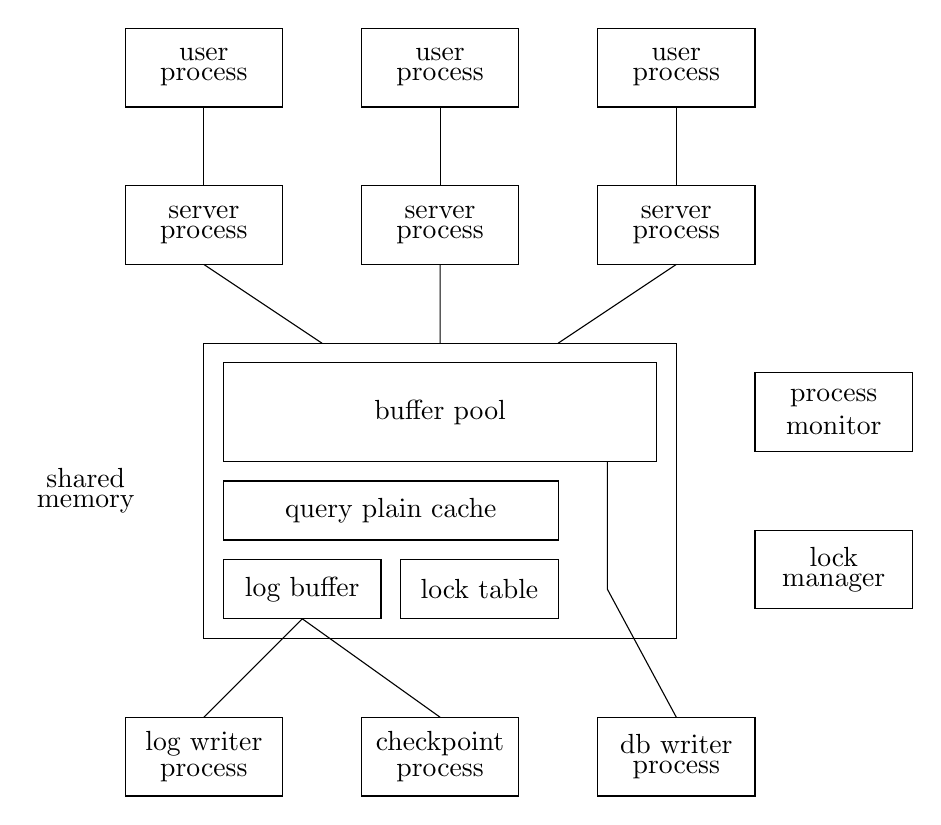
\begin{tikzpicture}
                    \foreach \x in {0, 3, 6} {
                        \node[] () at (\x + 1, -0.5) {\shortstack{user\\process}};
                        \node[] () at (\x + 1, -2.5) {\shortstack{server\\process}};
                        \draw
                        (\x, 0) -- (\x + 2, 0) -- (\x + 2, -1) -- (\x, -1) -- cycle
                        (\x, -2) -- (\x + 2, -2) -- (\x + 2, -3) -- (\x, -3) -- cycle
                        (\x + 1, -1) -- (\x + 1, -2);
                    }

                    \node[] () at (4, -4.875) {buffer pool};
                    \node[] () at (3.374, -6.125) {query plain cache};
                    \node[] () at (2.25, -7.125) {log buffer};
                    \node[] () at (4.5, -7.125) {lock table};
                    \draw
                    (1, -4) -- (7, -4) -- (7, -7.75) -- (1, -7.75) -- cycle
                    (1.25, -4.25) -- (6.75, -4.25) -- (6.75, -5.5) -- (1.25, -5.5) -- cycle
                    (1.25, -5.75) -- (5.5, -5.75) -- (5.5, -6.5) -- (1.25, -6.5) -- cycle
                    (1.25, -6.75) -- (3.25, -6.75) -- (3.25, -7.5) -- (1.25, -7.5) -- cycle
                    (3.5, -6.75) -- (5.5, -6.75) -- (5.5, -7.5) -- (3.5, -7.5) -- cycle;

                    \node[] () at (1, -9.25) {\shortstack{log writer\\process}};
                    \node[] () at (4, -9.25) {\shortstack{checkpoint\\process}};
                    \node[] () at (7, -9.25) {\shortstack{db writer\\process}};
                    \foreach \x in {0, 3, 6} {
                        \draw
                        (\x, -8.75) -- (\x + 2, -8.75) -- (\x + 2, -9.75) -- (\x, -9.75) -- cycle;
                    }
                    \draw
                    (1, -3) -- (2.5, -4)
                    (4, -3) -- (4, -4)
                    (7, -3) -- (5.5, -4)
                    (6.125, -5.5) -- (6.125, -7.125) -- (7, -8.75)
                    (2.25, -7.5) -- (1, -8.75)
                    (2.25, -7.5) -- (4, -8.75);

                    \node[] () at (-0.5, -5.875) {\shortstack{shared\\memory}};
                    \node[] () at (9, -4.875) {\shortstack{process\\monitor}};
                    \node[] () at (9, -6.875) {\shortstack{lock\\manager}};

                    \draw
                    (8, -5.375) -- (10, -5.375) -- (10, -4.375) -- (8, -4.375) -- cycle
                    (8, -7.375) -- (10, -7.375) -- (10, -6.375) -- (8, -6.375) -- cycle;
                \end{tikzpicture}
            \end{center}
            To ensure that multiple processes aren't accessing the same data, systems implement \textbf{mutual exclusion}, with either OS semaphores (controls access), or atomic instructions (test-and-set).
            \medskip

            We can classify physical storage based on the following factors;
            \begin{itemize}
                \itemsep0em
                \item access speed
                \item cost per unit of data
                \item reliability (data loss on system failure, and physical failure of storage)
            \end{itemize}
            The common types of physical storage used are as follows (ranked as a hierarchy);
            \begin{enumerate}[1.]
                \itemsep0em
                \item cache
                    \subitem fastest, and most costly - also volatile, and managed by the hardware
                \item main memory
                    \subitem fast access, but too small (or expensive) to store entire database - also volatile
                \item flash memory
                    \subitem non-volatile, and can survive power failure, data can be rewritten a limited number of times (10K - 1M cycles); fast reads, but slow writes, and erases
                \item flash memory (NOR)
                    \subitem fast reads, very slow erase, and low capacity
                \item flash memory (NAND)
                    \subitem high capacity
                \item magnetic disk
                    \subitem primary medium for long-term storage
                \item optical storage
                    \subitem reads, and writes slower than magnetic disk
                \item tape
                    \subitem extremely high capacity, primary used for backup (and archival data)
            \end{enumerate}
        \subsection*{Indexing}
            When we create an index (briefly mentioned above), it helps to speed up access to desired data. Another basic concept is the \textbf{search key}, which is an attribute used to look up records in a file. The index file consists of records, referred to as index entries, in the form \begin{tabular}{|c|c|}
                \hline
                search-key & pointer \\
                \hline
            \end{tabular}. The index files are typically much smaller than the original files. Indices are either ordered, where the search keys are stored in a sorted order, or search keys are distributed across "buckets" with a hash function.
            \subsubsection*{Ordered}
                In an ordered index, entries are sorted on the search key. In a sequentially ordered file, the primary index is the index whose search key specifies the order of the file (also referred to as a clustering index). This is usually the primary key. On the other hand, a secondary index is one whose search key specifies a different order from the sequential order of the file.
            \subsubsection*{Index Density}
                In a dense index, there is an index record for every search-key value in the file, as opposed to a sparse index file, where it only contains index records for some search key values. In order to find a record with the value $K$, we need to first find the index record with the largest search key, below $K$, and then search sequentially after that. A sparse index takes less space, and has less maintenance overhead for insertion and deletion, but is slower at locating records.
            \subsubsection*{Multilevel Index}
                If a primary index cannot fit in memory, access then becomes expensive. We can solve this by treating the primary index as a sequential file, and then creating another sparse index on it, where we have an outer index, which acts as a sparse index of the primary index, and the inner index being the original primary index file. The same process can be applied to the outer index if it's also too large to fit in memory, and so on. All levels must be updated on insertion, or deletion.

                \begin{center}
                    \begin{tikzpicture}[x=0.75cm, y=0.75cm]
                        \node[] () at (1, -4) {$\vdots$};
                        \node[] () at (6, -2.5) {$\vdots$};
                        \node[] () at (6, -6.5) {$\vdots$};
                        \node[] () at (1.5, -6.5) {outer index};
                        \node[] () at (6.5, -7.5) {inner index};
                        \draw
                        (0, 0) -- (3, 0) -- (3, -6) -- (0, -6) -- cycle
                        (2, 0) -- (2, -6)
                        (0, -1) -- (3, -1)
                        (0, -2) -- (3, -2);

                        \draw
                        (5, 0) -- (8, 0) -- (8, -3) -- (5, -3) -- cycle
                        (7, 0) -- (7, -3)
                        (5, -1) -- (8, -1)
                        (5, -2) -- (8, -2)
                        (5, -4) -- (8, -4) -- (8, -7) -- (5, -7) -- cycle
                        (7, -4) -- (7, -7)
                        (5, -5) -- (8, -5)
                        (5, -6) -- (8, -6);

                        \foreach \x in {0, -3, -6, -9} {
                            \draw
                            (10, \x) -- (13, \x) -- (13, \x - 2) -- (10, \x - 2) -- cycle;
                        }

                        \draw
                        (2.5, -0.5) edge[->] (5, -0.5)
                        (2.5, -1.5) -- (3.5, -1.5) edge[->] (5, -4.5)
                        (7.5, -0.5) edge[->] (10, -0.5)
                        (7.5, -1.5) -- (8.5, -1.5) edge[->] (10, -3.5)
                        (7.5, -4.5) -- (8.5, -4.5) edge[->] (10, -6.5)
                        (7.5, -6.5) -- (8.5, -6.5) edge[->] (10, -9.5);
                    \end{tikzpicture}
                \end{center}
            \subsubsection*{Record Deletion}
                If a deleted record was the only record in the file with the particular search-key value, the search-key value is deleted from the index (this is propagated across the multi-level index). In a dense index, the search-key deletion is similar to the file record deletion, but in a sparse index, if the value exists in the index, the value is replaced with the next search-key value in the file. If the value already exists in the index, the index record is deleted.
            \subsubsection*{Record Insertion}
                If the search-key value doesn't exist in the index, add it in (dense indices), on the other hand, with a sparse index, no change will be made, unless a new block has to be created. If a new block has to be created, the first search-key value in the block is inserted into the index. Multi-level insertion is done with the same process.
            \subsubsection*{Secondary Indices}
                I find it easier to consider this as a multi-level index, with the inner index being dense (therefore the index records points to a bucket that contains pointers to the actual records)
            \subsubsection*{B$^+$-Tree Index Files}
                Indexed-sequential files have some disadvantages in that the performance gets worse as the file gets bigger, since overflow blocks need to be created. Periodically, the entire file will also need to be reorganised. On the other hand, with B$^+$-tree index files, it can automatically reorganise itself with small changes when insertions, and deletions occur. However, there is additional overhead in insertion, deletion, as well as in space - but these disadvantages are outweighed by the advantages. The properties of a B$^+$-tree are as follows;
                \begin{itemize}
                    \itemsep0em
                    \item all paths from the root to leaf are of equal length
                    \item each node that is not a root, nor a leaf, has between $\ceil{\frac{n}{2}}$, and $n$ children
                    \item a leaf node has between $\ceil{\frac{n-1}{2}}$, and $n - 1$ values
                    \item if the root is not a leaf, then it has at least 2 children, otherwise if the root is a leaf (when there are no other nodes in the tree), it can have between 0, and $n - 1$ values
                \end{itemize}
                Pictured below is the structure of a typical node. We have $K_i$ as the search values, and $P_i$ are pointers to children (for non-leaf nodes), or pointers to records (or record buckets) when it is a leaf node. The keys are ordered $K_1 < K_2 < ... < K_{n - 1} $.
                \begin{center}
                    \begin{tabular}{|c|c|c|c|c|c|c|}
                        \hline
                        $P_1$ & $K_1$ & $P_2$ & ... & $P_{n - 1}$ & $K_{n - 1}$ & $P_n$ \\
                        \hline
                    \end{tabular}
                \end{center}
                $\forall i \in [1..n-1]$ the pointer $P_i$ either points to a file record with the search-key value $K_i$, or to a bucket of pointers, where all the pointers in the bucket have a search-key value of $K_i$. The bucket structure is only needed if the search-key doesn't form a primary key. If we have leaf nodes $L_i$, and $L_j$, and $i < j$, it follows that $L_i$'s search-key values are less than $L_j$'s search key values. $P_n$ points to the next leaf node, in the search-key order.
                \medskip

                On the other hand, non-leaf nodes form a multi-level sparse index on the leaf nodes. For a non-leaf node with $m$ pointers, all the search-keys in the subtree to which $P_1$ points, are less than $K_1$. $\forall i \in [2..n-1]$, all search-keys in the subtree to which $P_i$ points have values in the range $[K_{i-1}, K_i)$. All the search-keys in the subtree to which $P_n$ points to have values $\geq$ $K_{n - 1}$.
                \medskip

                We can find all records with a search-key value of ~k~ via the following method;
                \begin{lstlisting}
                    N = root
                    do
                        examine N for the smallest search-key value > k
                        if value exists
                            assume it is K$_\text{i}$
                            N = P$_\text{i}$
                        else it follows k >= K$_\text{n - 1}$
                            N = P$_\text{n}$
                    until N is a leaf node
                    if for some i, K$_\text{i}$ = k
                        follow pointer P$_\text{i}$ to record
                    else
                        no record with search-key value k exists
                \end{lstlisting}
                Note that at some point in the next paragraph I will start using S-K V, because I think this degree is giving me RSI.
                \medskip

                In order to insert values into the tree, we find the leaf node in which the value would appear. If the search-key value is already present, we add the record to the file, otherwise we add the record to the main file (and generate a bucket if needed). If there's room in the leaf node, insert the (key-value, pointer) pair in the leaf node, otherwise split the node. In order to split a leaf node, we take $n$ (S-K V, P) pairs, in a sorted order (including the pair being inserted). Place the first in the original node, and the rest in a new node. We then create a new pair ($k$, $p$), in the parent of the node being split. This is then propagated upwards if the parent is also full.
                \medskip

                To delete a record from the tree, we need to find the record and remove it from the main file (as well as from the bucket). Remove the pair from the leaf node, if the bucket becomes empty (or if there wasn't a bucket in the first place). If the node now has too few entries, and it is able to merge with a sibling to fit into a single node, we then merge siblings. This is done by inserting all the S-K Vs in the two nodes into a single node (the left-most one), and deleting the other. The deleted pair is then deleted from the parent, done recursively. However, if it cannot combine with a sibling, then we need to redistribute the pointers. Distribute it such that the number of pointers in both the current node, and the sibling node have more than the minimum number, and update the corresponding S-K V in the parent of the node.
                \medskip

                The index file degradation problem is solved by using indices, and the data file degradation problem is solved by the tree file organisation. The leaf nodes in a B$^+$-tree file organisation store records, instead of pointers. Since records are larger than pointers, the maximum number of records that can be stored in a leaf node is smaller than the number of pointers in a non-leaf node.
            \subsubsection*{Hashing}
                We can also use a hash function to obtain the bucket for a record, directly from it's S-K V. Given some hash function $h$, it maps the set of S-K Vs $K$ to the set of bucket addresses $B$. However, records with different S-K Vs can still be mapped to the same bucket, so the bucket will still need to be sequentially searched (however, on a smaller data set, provided the hash function is good). The worst hash function would map all S-K Vs to the same bucket, whereas an ideal function is uniform and assigns the same number to each bucket.
        \subsection*{NoSQL}
            However, due to the strong consistency needed for ACID transactions, it can be difficult to scale, especially because the idea of transactions was built into the optimisation of relational databases. Changing schema can also be difficult. One of the main objectives of NoSQL is to distribute the state, such that different objects are stored on different servers, by giving up ACID constraints, it can improve performance, we also give up strong consistency for eventual consistency. The key features of Not Only SQL / Not Relational are as follows;
            \begin{itemize}
                \itemsep0em
                \item horizontal scaling (more machines, instead of a more powerful machine)
                \item replicate / distribute data over servers
                \item simple call level interface
                \item weaker concurrency than ACID
                \item efficient use of main memory (and indices)
                \item flexible schema
            \end{itemize}
            NoSQL implementations can be split in to four categories; Key-Value, Graphs, BigTable, and Documents (nested values, like XML, or JSON).
            \subsubsection*{Key-Value}
                Think of it more as a file system than a database, and there is only a primary key (hence we lookup by key). Given some table of pairs, where the key $k_i$, has a corresponding value $v_i$, we have a simple API where lookup(key) leads to a value, lookup(key range) leads to a set of values, and so on. Insertion requires the pair, and deletion requires the key.
            \subsubsection*{Document Store}
                A pointerless object, and can have secondary indices, in addition to the KV stores.
            \subsubsection*{Column Family}
                Most implementations are based on Google's \textbf{BigTable}. It supports semi-structured data, is scalable, and is naturally indexed, however it's poor for interconnected data.
            \subsubsection*{Graph Databases}
                Modelled based on nodes, and relationships. Powerful data model, and general like RDBMS, easy to query, and connected data is indexed locally. A graph database has an explicit structure, where each node knows its adjacent nodes. The cost of a local step remains the same, even if the number of nodes increase.
\end{document}